\section{Experiments and Results}
\label{sec:experiments}

We evaluate Cylindrical Flow Matching on complex-valued MRI synthesis and downstream reconstruction using the raw $k$-space SKM-TEA-mini dataset \citep{desai2021skmtea} (single-coil, first-echo image space, comprising 3 complete 3D knee volumes with 1536 axial slices total). We partition the dataset into 2 patient volumes for training (1024 slices) and 1 completely held-out patient volume ($N=512$ contiguous slices) for testing. This constrained data regime provides a rigorous test of topological inductive bias: while Euclidean models must waste parameter capacity trying to approximate non-physical phase branch cuts, our cylindrical formulation natively respects $S^1 \times \mathbb{R}^+$ geometry, yielding superior generalization on unseen anatomy. Retrospective $4\times$ Cartesian undersampling is simulated using 1D phase-encoding masks with a central 24-line autocalibration signal (ACS) band, with exact Data Consistency ($\mathrm{DC\ Error} < 10^{-6}$) enforced via interleaved $k$-space projections.

\begin{figure}[!t]
    \centering
    \begin{subfigure}[t]{0.20\columnwidth}
        \centering
        {\scriptsize \textbf{(a) Ground Truth}}\\[1pt]
        {\tiny Reference}\\[2pt]
        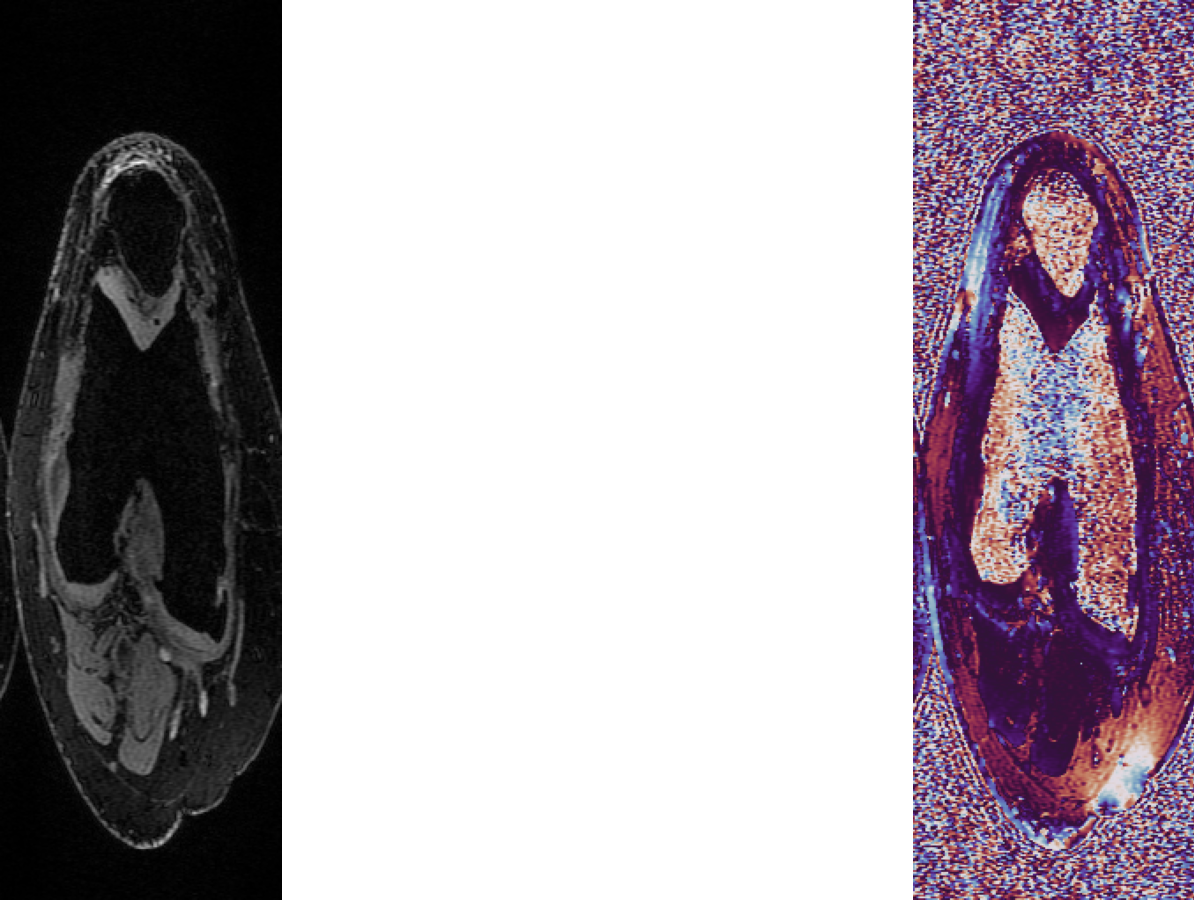
\includegraphics[width=\linewidth]{figures/panels/gt_pair.png}
    \end{subfigure}\hfill
    \begin{subfigure}[t]{0.39\columnwidth}
        \centering
        {\scriptsize \textbf{(b) Euclidean Flow} ($\mathbb{R}^2$)}\\[1pt]
        {\tiny 25.35 dB / 0.646 SSIM / 0.526 rad}\\[2pt]
        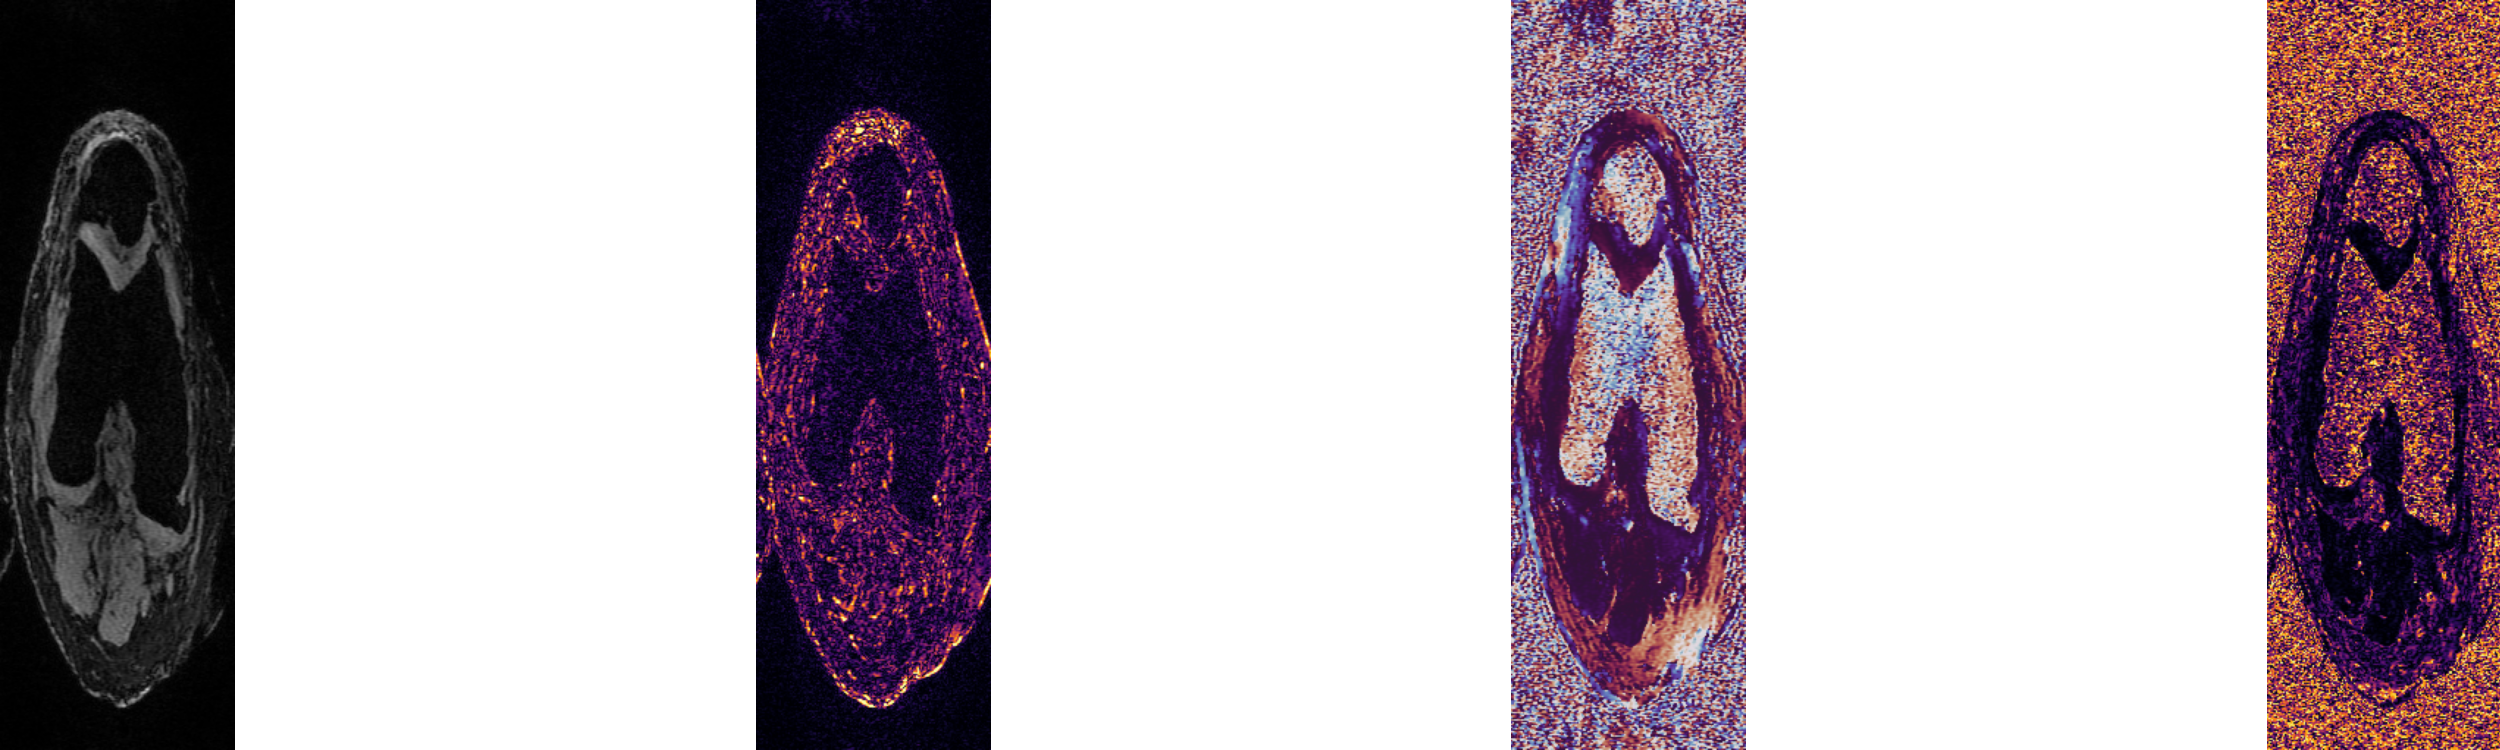
\includegraphics[width=\linewidth]{figures/panels/euc_quad.png}
    \end{subfigure}\hfill
    \begin{subfigure}[t]{0.39\columnwidth}
        \centering
        {\scriptsize \textbf{(c) Cylindrical Flow} (Ours)}\\[1pt]
        {\tiny \textbf{28.39 dB} / \textbf{0.762 SSIM} / \textbf{0.235 rad}}\\[2pt]
        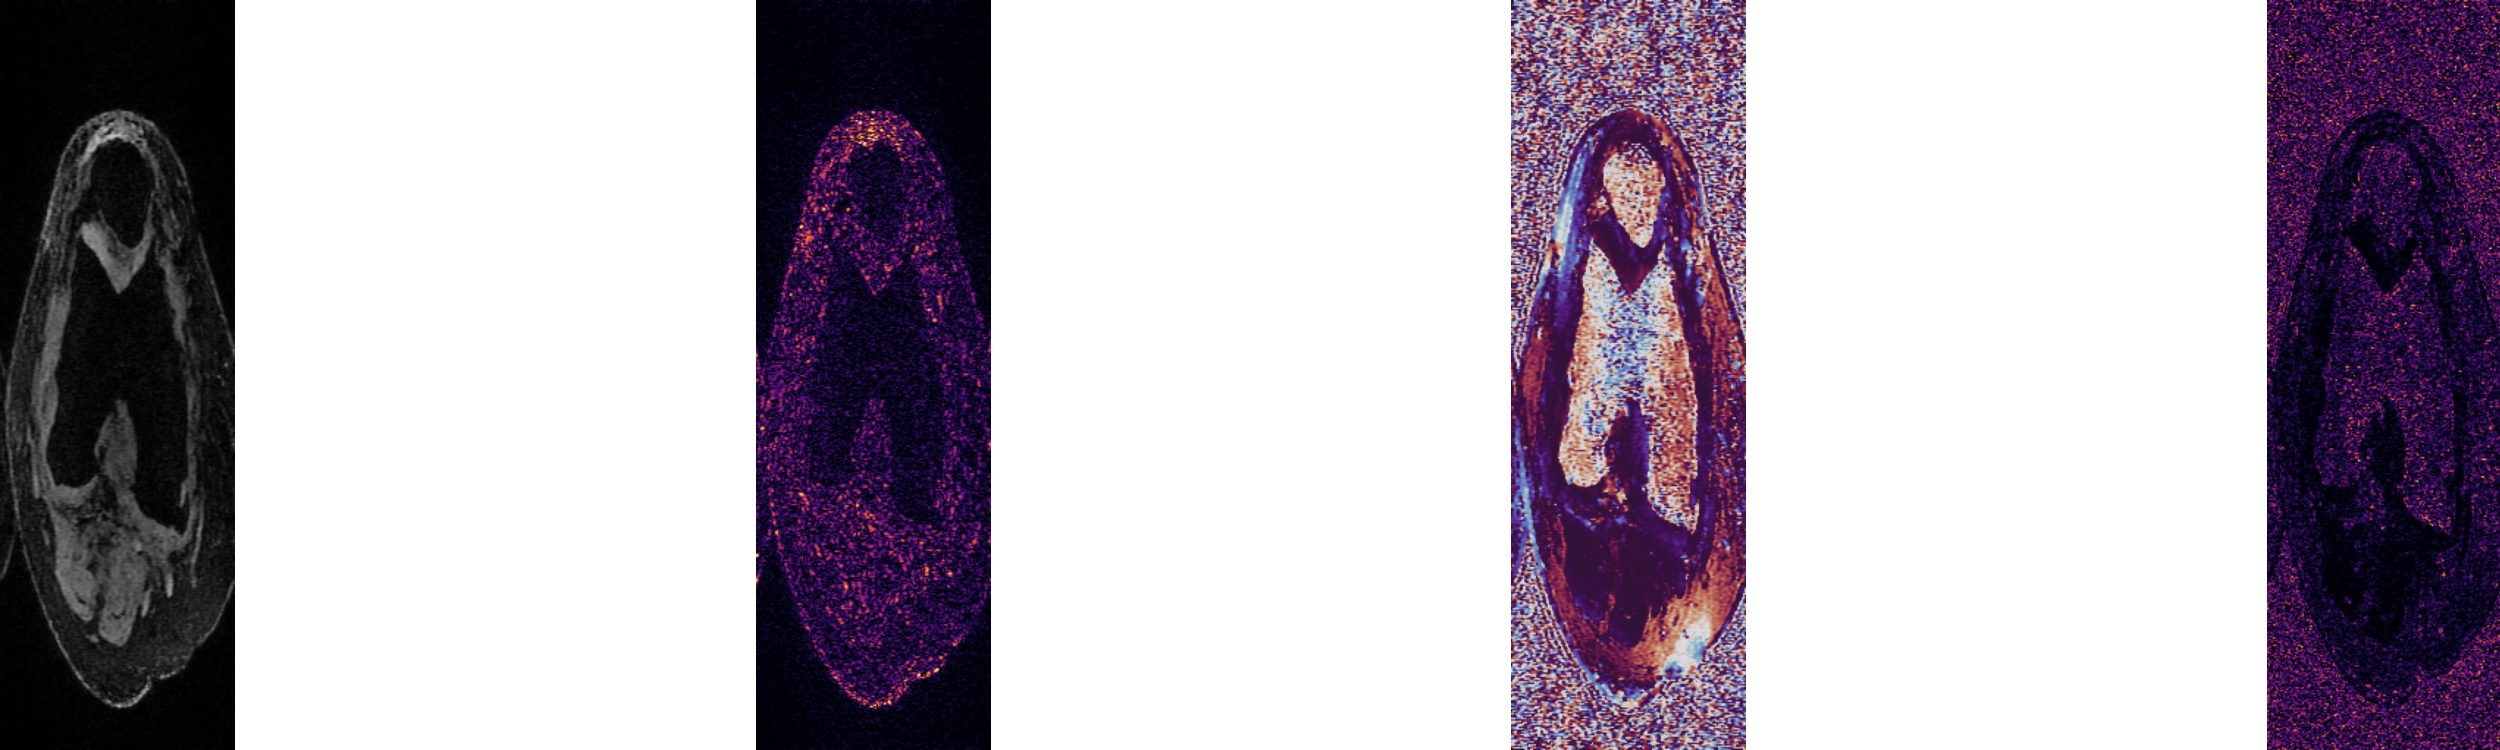
\includegraphics[width=\linewidth]{figures/panels/cyl_quad.png}
    \end{subfigure}
    \vspace{1mm}
    \caption{\textbf{Qualitative reconstruction on a representative held-out test slice.} Each method block displays (from left to right): reconstructed Amplitude, Amplitude Error $|\Delta A|$, reconstructed Phase, and Angular Phase Error $|\Delta\theta|$ (Ground Truth shows reference Amplitude and Phase). Test slice metrics are listed above each block. The Euclidean baseline exhibits severe phase seams and boundary magnitude cancellation, natively avoided by Cylindrical Flow.}
    \label{fig:results_visual}
    \vspace{-3mm}
\end{figure}

As shown in Figure \ref{fig:results_visual}, the Euclidean model struggles with phase wrapping, leading to artificial signal cancellations and magnitude dropouts near tissue boundaries (clearly highlighted in the residual error maps). In contrast, our geometry-aware approach explicitly models the $S^1$ phase topology, yielding continuous phase fields while preventing destructive interference, which results in significantly sharper anatomical reconstructions as evidenced across all quantitative metrics in Table \ref{tab:results_metrics}.

To evaluate phase fidelity, we compute the Circular Phase Error (CPE) in radians:
\begin{equation}
    \mathrm{CPE}(\theta, \hat{\theta}) = \frac{1}{|M|} \sum_{i \in M} |\operatorname{atan2}(\sin(\theta_i - \hat{\theta}_i),\, \cos(\theta_i - \hat{\theta}_i))|
\end{equation}
where $M$ denotes a tissue mask thresholded at $5\%$ of peak amplitude to avoid background noise bias.

\begin{table}[t]
    \centering
    \small
    \caption{\textbf{Quantitative metrics.} Descriptive evaluation across 512 contiguous slices of the held-out test volume ($4\times$ Cartesian reconstruction with exact Data Consistency projections).}
    \vspace{-1mm}
    \begin{tabular}{lccc}
        \toprule
        \textbf{Method} & \textbf{PSNR (dB) $\uparrow$} & \textbf{SSIM $\uparrow$} & \textbf{CPE (rad) $\downarrow$} \\
        \midrule
        Euclidean ($\mathbb{R}^2$) & 24.13 $\pm$ 1.18 & 0.530 $\pm$ 0.06 & 0.513 $\pm$ 0.07 \\
        \textbf{Cylindrical Flow (Ours)} & \textbf{24.47} $\pm$ \textbf{1.16} & \textbf{0.588} $\pm$ \textbf{0.04} & \textbf{0.405} $\pm$ \textbf{0.05} \\
        \bottomrule
    \end{tabular}
    \label{tab:results_metrics}
    \vspace{-2mm}
\end{table}
